\section{État de l'art}

\subsection{Introduction aux réseaux bayésien}
\label{IntroBN}

Un réseau bayésien est une distribution jointe de probabilité sur une famille \( (X_1,...,X_n) \) de variables aléatoires discrètes. Cette distribution est décrite par un \textit{graphe orienté sans circuit} ou DAG (Directed Acyclic Graph), et un ensemble de \textit{tables de probabilités conditionnelles} ou CPT (Conditional Probability Table). Les sommets du graphe représentent les variables aléatoires en question, et les arcs sont les dépendances conditionnelles entre les différentes variables.
\\
Dans un graphe orienté, on distingue trois types de relations entre un nœud \(\mathrm{X}\) et ses voisins, on dit que: 
\begin{itemize}
\centering
    \item \(\mathrm{Y}\) est un parent de \(\mathrm{X}\) si:  \quad\(\mathrm{Y} \rightarrow \mathrm{X} \)
    \item \(\mathrm{Z}\) est un enfant de \(\mathrm{X}\) si:  \quad\(\mathrm{Z} \leftarrow \mathrm{X} \)
    \item \(\mathrm{S}\) est une épouse de \(\mathrm{X}\) si:  \quad\(\mathrm{S} \rightarrow \mathrm{Z} \leftarrow \mathrm{X} \)
\end{itemize}

\noindent Où \(\mathrm{A} \rightarrow \mathrm{B} \) représente une arrête du noeud \(\mathrm{A}\) vers le noeud \(\mathrm{B}\). Dans ce dernier cas, \(\mathrm{S}\) est aussi un parent de \(\mathrm{Z}\). Les épouses sont définies comme des nœuds qui partagent au moins un enfant en commun et ne partageant entre eux aucun autre lien direct. (\cite{FouillesMassivesSoins})
\\
Ainsi, dans le cadre d'un réseau bayésien, si \(X_j\) est un parent de \(X_i\), alors \(X_i\) est dépendant de \(X_j\). En définissant \( Pa(X_i) \subseteq \{X_1,..., X_n\} \) comme l'ensemble des parent de \(X_i\), on retrouve \(P(X_i | Pa(X_i))\), la loi de \(X_i\) conditionnellement à l’état de ses parents \(Pa(X_i)\). C'est précisément cette loi que décrit le CPT associé au sommet de \(X_i\). Toutes les variables sont donc conditionnellement indépendante de leur non-descendant, sachant ses parents, on dit en autres qu'elles vérifient la \textit{propriété de Markov}. (\cite{gene_network})
\\
On retrouve ainsi la probabilité jointe de la famille \((X_1,..., X_n)\) de variables aléatoires par la formule des probabilités composées:
\begin{equation}
\label{eq:1}
    P(X_1,..., X_n) = \prod_{i=1}^{n}P(X_i | Pa(X_i))
\end{equation}
Un avantage capital des réseaux bayésiens se trouve dans leur capacité à représenter de manière succincte des distributions multidimensionnelles, sans tomber dans l'explosion combinatoire. En effet, en passant par une étude de graphes, le nombre de paramètre à calculer est réduit conséquemment grâce à la factorisation (\ref{eq:1}).
\begin{figure}
\centering
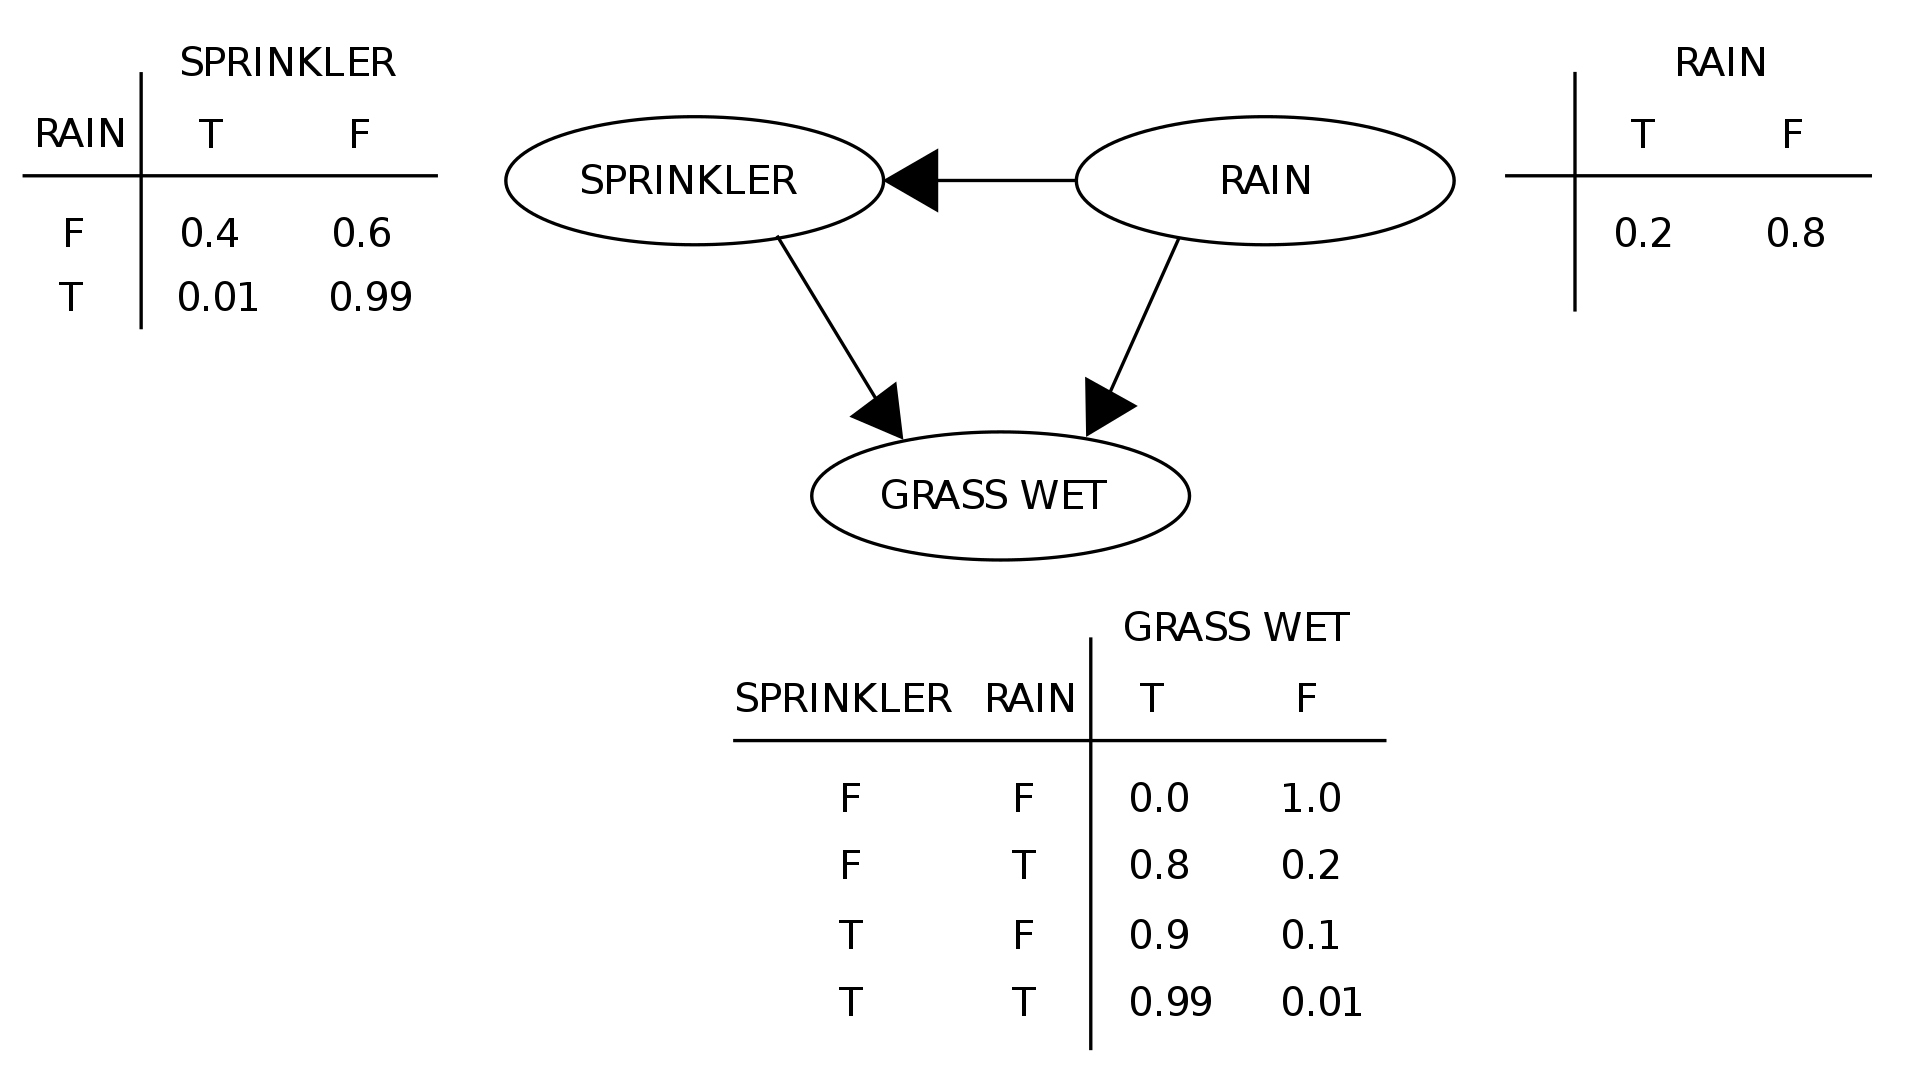
\includegraphics[scale=0.18]{SimpleBayesNet.png}
\caption{Exemple d'un réseau bayésien avec trois arrêtes}
\label{fig:ExBN}
\end{figure}
%Dans l'exemple de la figure \ref{fig:ExBN}, 

\subsection{Introduction à l'informatique quantique}
\label{IntroQuant}

Similairement au bit de la théorie de l’information classique, l’information quantique se base sur la manipulation de bits quantiques, appelés \textit{qubits}. Cependant, l’espace d’état de ces derniers diffère de leur homologue classique dû au fait que nous retrouvons, en plus des états \(0\) et \(1\), les états de superposition, dans lesquelles les qubits en question peuvent être dans les deux états simultanément avant d’être mesurés (ou observés). En pratique, les qubits sont représentés par les vecteurs unitaires de \(\mathbb{C}^2 \) muni du produit scalaire hermitien. L’état \(|0\rangle\), représenté par le vecteur \((1\;0)\) et l’état \(|1\rangle\) par \((0\;1)\), sont les bits classiques et forment la base canonique de l’espace vectoriel. 
\\
Tout qubit \(|\psi\rangle\) s’exprime donc par une combinaison linéaire : 
\begin{equation}
|\psi\rangle = \alpha|0\rangle +\beta|1\rangle \quad \text{tel que} \quad (\alpha,\beta) \in \mathbb{C}^2 , \; |\alpha|^2 + |\beta|^2 = 1
\end{equation}

\noindent La mesure d’un qubit entraîne le phénomène de réduction, qui réduit un qubit superposée en un bit classique, elle entraîne en outre la destruction de l’information quantique contenu dans le qubit. Le module au carré de chacune des deux coordonnées du qubit dans \(\mathbb{C}^2 \) représente ainsi les probabilités respectives de \(0\) et \(1\) lors de la mesure, ce qui illustre le principe de superposition. D’un point du vue probabiliste, le fait que le vecteur du qubit soit unitaire nous assure que les probabilités associées aux états classiques forment un système complet d'événements. Géométriquement, la visualisation d’un qubit se fait à travers la sphère de Bloch, celle-ci permet d’étudier les qubits du plan \(\mathbb{C}^2 \) sous la structure algébrique de \(\mathbb{R}^3 \) en utilisant les coordonnées sphériques. 
\\
\begin{figure}
\centering
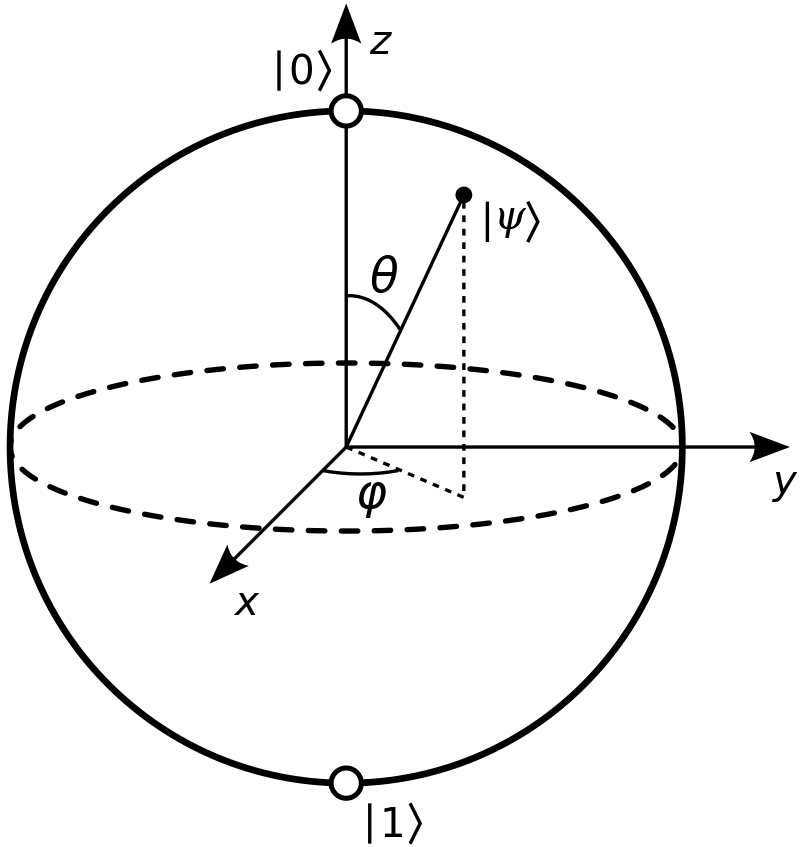
\includegraphics[scale=0.15]{Bloch_sphere.png}
\caption{La Sphère de Bloch}
\label{fig:Bloch}
\end{figure}
\noindent Nous développerons ici des algorithmes quantiques sous le modèle de circuits quantiques, qui réalisent les opérations sur les qubits séquentiellement. Ces opérations sont effectuées par les portes quantiques représentées par les opérateurs unitaires de \(\mathbb{C}^2 \) sous la forme de \(U(\theta, \phi, \lambda)\), qui sont analogues aux portes logiques pour les circuits électroniques classiques. On retrouve notamment la porte NOT ou \(X\), mais aussi \(R_Y\) et \(R_Z\) qui représentent une rotation selon l’axe X, Y et Z respectivement dans la sphère de Bloch, celles-ci sont aussi appelées \textit{portes de rotations}. (\cite{quant_rep_BN})
\begin{equation}
\mathrm{U}(\theta, \phi, \lambda) = 
\begin{bmatrix}
cos(\frac{\theta}{2}) & -e^{i\lambda}sin(\frac{\theta}{2}) \\
e^{i\phi}sin(\frac{\theta}{2}) & e^{i(\phi + \lambda)}cos(\frac{\theta}{2})
\end{bmatrix}
, \quad 
(\theta, \phi, \lambda) \in [0,\pi] \times [0, 2\pi]^2
\end{equation}
Pour réaliser des opérations concernant de multiples qubits, nous faisons recours au \textit{produit tensoriel}, qui est un moyen commode de coder les objets multilinéaires. En pratique, les portes $X$ et $R_Y$ contrôlée ($CNOT$ et $CR_Y$) seront utilisées principalement. Celles-ci agissent sur un qubit de contrôle et un qubit cible ; quand le qubit de contrôle vaut \(0\), le qubit cible reste inchangée, tandis que lorsqu’il vaut \(1\), la porte \(X\) (ou $R_Y$) est appliquée sur le qubit cible. Il est possible d’exprimer la version contrôlée d’une opération unitaire \(U\) quelconque comme une combinaison de porte \(CX\) et de porte agissant sur un seul qubit. Plus généralement, ces opérations engendrent les portes 
\(C^nU\)  ayant n qubits de contrôle et un qubit cible. Celles-ci appliquent l’opération \(U\) sur le qubit cible lorsque tous les n-qubits valent \(1\), et constituent toutes les opérations que nous utiliserons dans ce projet.

\begin{equation}
CX = 
\begin{bmatrix}
1&0&0&0\\
0&1&0&0\\
0&0&0&1\\
0&0&1&0\\
\end{bmatrix}
, \quad 
CU = 
\begin{bmatrix}
1&0&0&0\\
0&1&0&0\\
0&0&cos(\frac{\theta}{2}) & -e^{i\lambda}sin(\frac{\theta}{2}) \\
0&0&e^{i\phi}sin(\frac{\theta}{2}) & e^{i(\phi + \lambda)}cos(\frac{\theta}{2})
\end{bmatrix}
\end{equation}


\subsection{Approche à un problème NP-difficile}
\label{QuantRepBN}


Le cadre du projet se porte sur l'inférence dans les réseaux bayésien, c'est-à-dire la détermination de la probabilité postérieure d'un ensemble de variables étant donné certaines observations. L'inférence exacte requiert dans les pires des cas une sommation sur un nombre exponentiel de configurations de variables, il s'agit d'un problème \textit{NP-difficile}.\footnotemark
\\
L'exploration exhaustive des configurations structurelles possibles contraintes par un critère d'optimisation tel que la vraisemblance, devient rapidement une tâche herculéenne. À mesure que le nombre de variables s'accroît, il y a une augmentation exponentielle du nombre de structures à évaluer, rendant ainsi le processus de sélection impraticable. Afin de tirer avantage des temps de calcul réduits des ordinateurs quantiques, nous allons construire des circuits quantiques qui représenteront des réseaux bayésien afin d'évaluer leur performances inférentielles.
\\
Plus concrètement, nous aborderons le problème d'inférence à travers 
l'échantillonnage par rejet avec la méthode de Monte-Carlo. Pour un réseau 
bayésien à $k$ variables ayant chacune moins de $m$ parents, la génération d’échantillons classiques de la loi jointe se fait en $\mathcal{O}(km)$. Ainsi pour $P_e$ la probabilité de l’observation, la méthode de rejet possède une complexité en espérance de $\mathcal{O}(km/P_e)$. La performance computationnelle de l’algorithme classique se dégrade des lorsque $P_e$ devient faible, c'est-à dire lorsque le nombre de variables observées augmente.
\\
Notre objectif est donc de reformuler la problématique d'échantillonnage en un problème pour lequel l'algorithmique quantique présente un avantage considérable : la recherche non structurée, pour obtenir une complexité finale de $\mathcal{O}(k2^m/\sqrt{P_e})$. 


\footnotetext{Dans la théorie de la complexité informatique, la classe de problème non déterministe polynomial NP contient les problèmes dont on peut vérifier si une solution est candidate en temps polynomial. On dit alors qu'un problème H est NP-difficile, si tout problème L de la classe NP peut être réduit en temps polynomial à H. C'est-a-dire on peut transformer en temps polynomial, la résolution de H en résolutions de problèmes NP.}